%! TeX program = lualatex
\documentclass{tp}
\usepackage{mhchem}
\titre{TP29 : Diagramme potentiel-pH}
\begin{document}
%\small


\section{Objectif du TP}
L'objectif de ce TP est de tracer le diagramme potentiel-pH correspondant au couples Fer(III)/Fer(II) et de l'utiliser pour prévoir les réactions d'oxydoréduction métant en jeu les éléments fer et iode.

\section{Montage expérimental et mesures}%
\label{sec:montage_experimental_et_mesures}

Le montage expérimental utilisé dans ce TP pour faire l’acquisition de diagrammes potentiel-pH est présenté sur la figure ci-dessous. L’électrode de référence  est directement reliée au pHmètre/Voltmètre. L’électrode de platine (on voit le fil de platine) sert à mesurer le potentiel de la solution, tandis que la troisième électrode, électrode de verre, sert à la mesure du pH. Ces trois électrodes doivent plonger dans la solution à étudier.

\begin{center}
  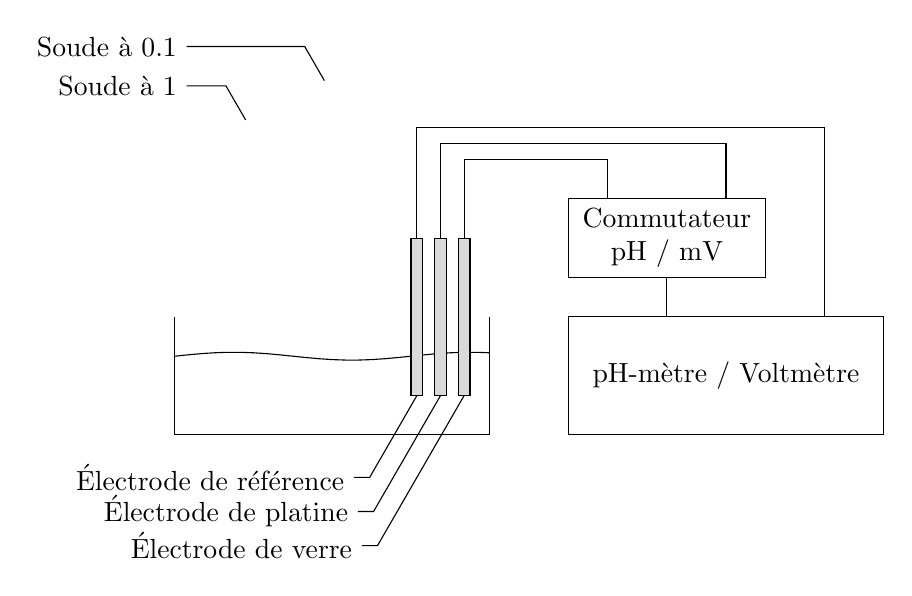
\begin{tikzpicture}
    \burette{{(0,1.5)}}
    \draw (-0.1, 4) -- ++(120:0.5) --++(-0.5, 0) node[left]{Soude à \SI{1}{\mol\per\litre}} ;
    \burette{{(1,1.5)}}
    \draw (0.9, 4.5) -- ++(120:0.5) --++(-1.5, 0) node[left]{Soude à \SI{0.1}{\mol\per\litre}} ;
    \draw (-1, 1.5) -- ++(0, -1.5) -- ++(4, 0) -- ++(0,1.5);
    \draw (-1, 1) plot[domain=0:4] (\x-1, {1+0.05*sin(120*\x)});
    \draw[fill=gray!30] (2, 0.5) coordinate (D) rectangle ++(0.15, 2) coordinate (A);
    \draw[fill=gray!30] (2.3, 0.5) coordinate (E) rectangle ++(0.15, 2) coordinate (B);
    \draw[fill=gray!30] (2.6, 0.5) coordinate (F) rectangle ++(0.15, 2) coordinate (C);

    \draw (4, 0) rectangle ++(4, 1.5) node[midway]{pH-mètre / Voltmètre};
    \draw (4, 2) rectangle ++(2.5, 1) node[midway, align=center]{Commutateur\\pH / mV};

    \draw (C) ++(-0.075, 0) |- (4.5, 3.5) -- (4.5, 3) ;
    \draw (B) ++(-0.075, 0) |- (6, 3.7) -- (6, 3) ;
    \draw (A) ++(-0.075, 0) |- (7.25, 3.9) -- (7.25, 1.5) ;
    \draw (5.25, 2) -- (5.25, 1.5);

    \draw (D) ++(0.075, 0) -- ++(-120:1.2) -- ++(-0.2, 0) node[left] {Électrode de référence} ;
    \draw (E) ++(0.075, 0) -- ++(-120:1.7) -- ++(-0.2, 0) node[left] {Électrode de platine} ;
    \draw (F) ++(0.075, 0) -- ++(-120:2.2) -- ++(-0.2, 0) node[left] {Électrode de verre} ;
  \end{tikzpicture}
  \captionof{figure}{Schéma du montage expérimental}
\end{center}

Les deux électrodes de mesure (platine et verre) sont reliées au pH-mètre/Voltmètre par l'intermédiaire d'un commutateur qui permet de sélectionner l'une ou l'autre. Il faut que le mode de mesure du pH-mètre (pH ou mV) soit cohérent avec l'électrode sélectionnée par le commutateur.

Deux burette graduées permette d'ajouter de la soude à \SI{1}{\mol\per\litre} ou de la soude à \SI{0.1}{\mol\per\litre}.

\begin{itemize}
  \item Étalonner le pH-mètre avec les solutions tampon.
  \item Verser \SI{100}{\milli\litre} de la solution contenant les ions \ce{Fe^3+}/\ce{Fe^2+} dans un bécher de \SI{250}{\milli\litre}.

  \item Plongere les trois électrodes dans la solution.

  \item Faire une dilution par 10 de la soude à \SI{1}{\mol\per\litre} pour obtenir une solution de soude à \SI{0.1}{\mol\per\litre}. Remplir les deux burettes graduées avec les deux solutions de soude.

  \item Faire varier le pH (par pas d'environ \num{0.5}) et noter la valeur du potentiel de la solution pour chaque valeur de pH. Pour faire varier le pH, ajouter de la soude à \SI{1}{\mol\per\litre} jusqu'à pH=3, puis de la soude à \SI{0.1}{\mol\per\litre} jusqu'à pH=8, puis de la soude à \SI{1}{\mol\per\litre} jusqu'au pH le plus élevé possible (burette vide). Relever les pH d'apparition des précipités. 
\end{itemize}

\section{Exploitation des mesures}%
\label{sec:exploitation_des_mesures}

\begin{itemize}
  \item Déterminer la pente des droites modélisant les résultats expérimentaux dans les trois domaines de pH que l'on mettra en évidence.

  \item Déterminer les valeurs théoriques du pH de début de précipitation de l'hydroxyde ferreux \ce{Fe(OH)2} et de l'hydroxyde ferrique \ce{Fe(OH)3}.

  \item En déduire l'expression théorique du potentiel $E$ de cette solution en fonction du pH. 

  \item Comparer les pentes des droites aux pentes théoriques.

  \item Pourquoi la solution initiale est-elle acidifiée ?
\end{itemize}

Mélanger \SI{20}{\milli\litre} d'une solution de chlorure ferrique avec \SI{20}{\milli\litre} d'une solution d'iodure de potassium.

\begin{itemize}
  \item Qu'observe-t-on ? Interpréter en utilisant le diagramme potentiel-pH tracé précédemment.
\end{itemize}

Ajouter progressivement de la soude à \SI{1}{\mol\per\litre} à la solution précédente. 

\begin{itemize}
  \item Qu'observe-t-on ? interpréter.
\end{itemize}

On donne à \SI{25}{\celsius} : 
\begin{itemize}
  \item $E^\circ(\ce{I2(aq) / I-})=\SI{0.54}{\volt} $ ;
  \item $E^\circ(\ce{Fe^3+ / Fe^2+})=\SI{0.77}{\volt} $ ;
  \item $\mathrm{p}K_s(\ce{Fe(OH)2})=\num{15}$ ;
  \item $\mathrm{p}K_s(\ce{Fe(OH)3})=\num{38}$.
    \item Potentiels des différentes électrodes de référence :
\begin{itemize}
  \item électrode au calomel $E_\text{ref}=\SI{0.241}{\volt}$ ;
  \item électrode d'argent (la plus probable) $E_\text{ref}=\SI{0.225}{\volt}$;
  \item électrode au sulfate mercureux  (la moins probable) $E_\text{ref}=\SI{0.651}{\volt}$. 
\end{itemize}
\end{itemize}


\end{document}

